

\tikzset{every picture/.style={line width=0.75pt}} %set default line width to 0.75pt        

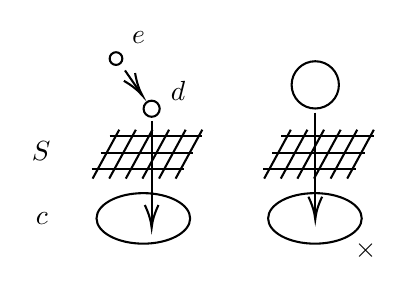
\begin{tikzpicture}[x=0.75pt,y=0.75pt,yscale=-1,xscale=1]
%uncomment if require: \path (0,300); %set diagram left start at 0, and has height of 300

%Shape: Ellipse [id:dp10401378338786049] 
\draw   (74,113.39) .. controls (74,106.67) and (84.1,101.22) .. (96.56,101.22) .. controls (109.01,101.22) and (119.11,106.67) .. (119.11,113.39) .. controls (119.11,120.11) and (109.01,125.56) .. (96.56,125.56) .. controls (84.1,125.56) and (74,120.11) .. (74,113.39) -- cycle ;
%Shape: Grid [id:dp09583060841478219] 
\draw  [draw opacity=0] (81.95,70.67) -- (126.56,70.67) -- (113.72,94.22) -- (69.11,94.22) -- cycle ; \draw   (84.95,70.67) -- (72.11,94.22)(92.95,70.67) -- (80.11,94.22)(100.95,70.67) -- (88.11,94.22)(108.95,70.67) -- (96.11,94.22)(116.95,70.67) -- (104.11,94.22)(124.95,70.67) -- (112.11,94.22) ; \draw   (80.31,73.67) -- (124.92,73.67)(75.95,81.67) -- (120.56,81.67)(71.59,89.67) -- (116.2,89.67) ; \draw    ;
%Shape: Circle [id:dp31189924819685966] 
\draw   (80.33,36.39) .. controls (80.33,34.7) and (81.7,33.33) .. (83.39,33.33) .. controls (85.08,33.33) and (86.44,34.7) .. (86.44,36.39) .. controls (86.44,38.08) and (85.08,39.44) .. (83.39,39.44) .. controls (81.7,39.44) and (80.33,38.08) .. (80.33,36.39) -- cycle ;
%Straight Lines [id:da12935033787340267] 
\draw    (87.72,42.11) -- (94.97,52.58) ;
\draw [shift={(96.11,54.22)}, rotate = 235.29] [color={rgb, 255:red, 0; green, 0; blue, 0 }  ][line width=0.75]    (10.93,-3.29) .. controls (6.95,-1.4) and (3.31,-0.3) .. (0,0) .. controls (3.31,0.3) and (6.95,1.4) .. (10.93,3.29)   ;
%Shape: Circle [id:dp7222065551952845] 
\draw   (96.67,60.56) .. controls (96.67,58.41) and (98.41,56.67) .. (100.56,56.67) .. controls (102.7,56.67) and (104.44,58.41) .. (104.44,60.56) .. controls (104.44,62.7) and (102.7,64.44) .. (100.56,64.44) .. controls (98.41,64.44) and (96.67,62.7) .. (96.67,60.56) -- cycle ;
%Straight Lines [id:da7276461675375434] 
\draw    (100.56,66.44) -- (100.56,115.89) ;
\draw [shift={(100.56,117.89)}, rotate = 270] [color={rgb, 255:red, 0; green, 0; blue, 0 }  ][line width=0.75]    (10.93,-3.29) .. controls (6.95,-1.4) and (3.31,-0.3) .. (0,0) .. controls (3.31,0.3) and (6.95,1.4) .. (10.93,3.29)   ;
%Shape: Ellipse [id:dp12697611260252684] 
\draw   (156.67,113.39) .. controls (156.67,106.67) and (166.77,101.22) .. (179.22,101.22) .. controls (191.68,101.22) and (201.78,106.67) .. (201.78,113.39) .. controls (201.78,120.11) and (191.68,125.56) .. (179.22,125.56) .. controls (166.77,125.56) and (156.67,120.11) .. (156.67,113.39) -- cycle ;
%Shape: Grid [id:dp9936460967678797] 
\draw  [draw opacity=0] (164.61,70.67) -- (209.22,70.67) -- (196.39,94.22) -- (151.78,94.22) -- cycle ; \draw   (167.61,70.67) -- (154.78,94.22)(175.61,70.67) -- (162.78,94.22)(183.61,70.67) -- (170.78,94.22)(191.61,70.67) -- (178.78,94.22)(199.61,70.67) -- (186.78,94.22)(207.61,70.67) -- (194.78,94.22) ; \draw   (162.98,73.67) -- (207.59,73.67)(158.62,81.67) -- (203.23,81.67)(154.26,89.67) -- (198.87,89.67) ; \draw    ;
%Shape: Circle [id:dp838751100400853] 
\draw   (168,49.06) .. controls (168,42.77) and (173.1,37.67) .. (179.39,37.67) .. controls (185.68,37.67) and (190.78,42.77) .. (190.78,49.06) .. controls (190.78,55.35) and (185.68,60.44) .. (179.39,60.44) .. controls (173.1,60.44) and (168,55.35) .. (168,49.06) -- cycle ;
%Straight Lines [id:da5932706956135338] 
\draw    (179.39,62.44) -- (179.39,111.89) ;
\draw [shift={(179.39,113.89)}, rotate = 270] [color={rgb, 255:red, 0; green, 0; blue, 0 }  ][line width=0.75]    (10.93,-3.29) .. controls (6.95,-1.4) and (3.31,-0.3) .. (0,0) .. controls (3.31,0.3) and (6.95,1.4) .. (10.93,3.29)   ;

% Text Node
\draw (43.33,109) node [anchor=north west][inner sep=0.75pt]   [align=left] {$\displaystyle c$};
% Text Node
\draw (41.33,75) node [anchor=north west][inner sep=0.75pt]   [align=left] {$\displaystyle S$};
% Text Node
\draw (113,123.67) node [anchor=north west][inner sep=0.75pt]   [align=left] {$\displaystyle \checkmark$};
% Text Node
\draw (197,123) node [anchor=north west][inner sep=0.75pt]   [align=left] {$\displaystyle \times $};
% Text Node
\draw (108.33,46) node [anchor=north west][inner sep=0.75pt]   [align=left] {$\displaystyle d$};
% Text Node
\draw (89.67,22) node [anchor=north west][inner sep=0.75pt]   [align=left] {$\displaystyle e$};


\end{tikzpicture}